% #############################################################################
% This is Chapter 6
% !TEX root = ../main.tex
% #############################################################################
% Change the Name of the Chapter i the following line
\fancychapter{Methodology}
% The following line allows to ref this chapter
\label{chap:methd}

This chapter discusses the evolutions of the pipeline against the baseline methodology and covers the methodology itself in detail. Using \ac{GenAI} as a method implementation support tool accelerates development substantially, but sheds light on some issues that need to be addressed in order for \ac{GenAI} to be helpful instead of hindering progress. These issues are discussed in the \ref{MethodEvo} section. Afterwards, each step of the methodology is covered in detail during section \ref{methodPipeline}, with a detailed explanation of the task the \ac{LLM} accompanying the user performs. Throughout the process, multiple confirmation gates are presented to the user to allow as much control of the output as possible.

% #############################################################################
\section{Method Evolution} 
\label{MethodEvo}

During development and testing of the methodology, specific pipeline stages presented significant shortcomings that demanded resolution. These phases were namely the ``Regulatory Relevance Analysis'' and all the steps that materialized Views (``Contextualized Regulation Overview Baseline'' and ``View Generation''). 

Regulatory relevance analysis proved difficult due to the relative interpretation of legal text in conjunction to the non-deterministic nature of \ac{LLM}s. Sometimes agents would identify some laws as being relevant to the designated stakeholder and sometimes they would not. 

View materialization required two distinct hurdles be surpassed. Due to \ac{LLM}s having no real spatial awareness, produced Archimate diagrams were cluttered and relations crossed each other multiple times as well as crossing other elements. This resulted in an unreadable view. Therefore, spatial organization and positioning of elements was made agnostic to the \ac{LLM}. It can't fail at a task that is not within scope.
Besides view organization, \ac{GenAI} also struggled to develop the \ac{XML} properly. The \ac{XML} behind an archi model is a very extensive document. If an \ac{XML} is very deeply nested, the \ac{LLM} may ``forget'' the exact opening tag by the time they need to close it, resulting in malformed syntax. In addition to this, the verbosity of \ac{XML} increases the generation length, which in turn increases the probability that the model will ``hallucinate'' or make a structural error somewhere during generation. Due to this, most of the times, the generated Archimate file would not even be syntactically valid .

\subsection{Excel Traceability Matrix}
\label{traceMatrixEvo}

The Excel Traceability Matrix evolved from a manual process to a fully automated one. This means that the time invested to get the Matrix ready diminished from two hours all the way down to a few seconds. A small program was created using \texttt{C\#} that analyses the \ac{HTML} from the target legislation, and outputs the Traceability Matrix without any human input.

Besides automation for the sake of efficiency, the traceability matrix also suffered a complete redesign to improve readability. As can be observed on the extract from the baseline Traceability Matrix on \ref{tab:traceMatrix}, the \ac{ID} system is not intuitive. This is because the different \ac{ID}s can mean any of the sub-article levels, which are not explained anywhere in the matrix. Additionally, of all the groupings referred in section \ref{sec:legisStruc}, only Chapters are mentioned. To address this, every possible grouping that a a legislative text may have exists as an \ac{ID} column. An excerpt of the new traceability matrix can be observed in \ref{tab:newTraceMatrix}.

\begin{figure}[H]
    \centering
    % Use \includegraphics to load the screenshot of your table
    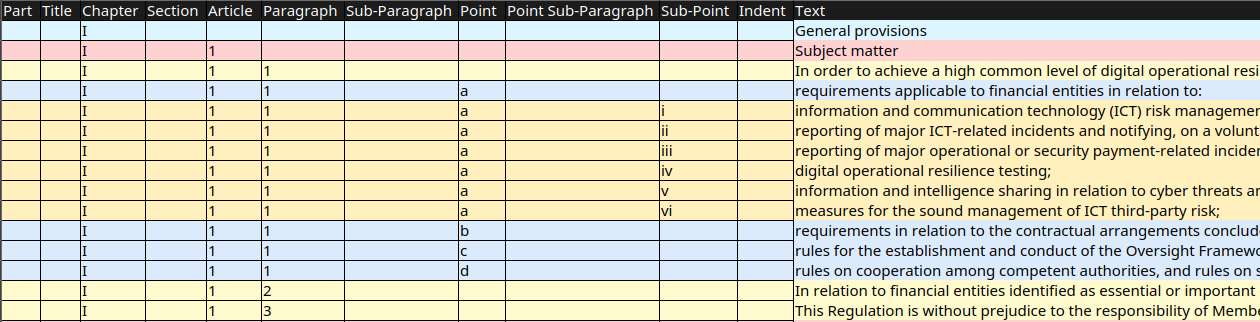
\includegraphics[width=1\textwidth]{Images/DoraTraceMatrixExcerpt.png} 
    \caption{Sample from the traceability matrix of \ac{DORA} generated by the traceability matrix creator program}
    \label{tab:newTraceMatrix}
\end{figure}


\subsection{Diagram as Code}

Using ``Diagram as Code'' made the \ac{LLM} agnostic to both the verbosity of the \ac{XML} syntax as well as the positioning of elements. This approach already proved to achieve very good results. Examples of this are Mermaid and LikeC4, with the latter being a closer relative to ArchiMate, built around the concept of an architectural model and not independent visual drawings. Archimate, however, does not fit into this category, since it is a standardized modelling language, not a diagramming method. The approach can, however, be applied to Archimate trough the usage of pyArchimate. This way, the \ac{LLM} only has to write python code responsible for the generation of the Archimate \ac{XML}. This never fails syntactically, element positioning is made simpler to the \ac{LLM} and the model only has to handle a program that, compared to the resulting \ac{XML}, is a fraction of the size.

\subsection{Legal Text Interpretation}

The relativity of interpreting legal text was mitigated trough the use of an agentive debate panel, made up of a moderator and three legislative evaluators. Each evaluator looks at the legislation trough a different lens, and confronts it against the stakeholder's operational footprint, taking note of what is deemed relevant for the stakeholder. The lenses in question are the literal (identifies requirements that explicitly match the stakeholder's documented responsibilities), systemic (takes into account dependencies between systems, teams and processes that may make a legal requirement relevant) and gap (looks for operational weaknesses and missing controls where the law may expose an unresolved gap). The panel then debates on what should be included in the final report, and the moderator collects the unanimous decisions as well as the ones that did not pass, but had some votes in favour. Everything decided is subject to user approval before being materialized to file. The step-by-step operation of the panel is detailed in table \ref{tab:PanelSteps} 

\begin{table}[htbp]
\centering
\caption{Order of agentive debate panel}
\label{tab:PanelSteps}

\begin{tabular}{p{0.15\textwidth} p{0.78\textwidth}}
\hline
\textbf{Step} & \textbf{Action} \\
\hline
1 & Launch the Literal, Systemic, and Gap Evaluator agents concurrently for independent regulatory evaluations. \\

2 & The Moderator compiles the evaluators' initial proposal matrix. \\

3 & The Moderator presents peer proposals and re-invokes the evaluators for multi-turn debate. \\

4 & Retain only the articles on which all three evaluators explicitly agree. \\

5 & The Moderator synthesizes the operational justifications and exhaustive statutory requirements. \\

6 & Obtain user approval, generate the traceability matrix, and validate it. \\

7 & Resolve each in-scope duty to its exact canonical legal-text identifier. \\

8 & Build the bidirectional stakeholder--regulation Coverage Ledger. \\

9 & Creates approved coverage relationships. \\

10 & Map the stakeholder, employing organization, and law-defined legal-role group. \\

11 & Check if user approves Relevant Articles, Omitted Articles, Traceability Matrix, Legal Text IDs, Coverage Resolution and Stakeholder Legal Role \\

12 & Persist the approved report as \texttt{5\_regulatory\_relevance.md}. \\
\hline
\end{tabular}
\end{table}
\FloatBarrier

To test if the panel did in-fact cause output to be consistent through-out different iterations (thus confirming \texttt{R3}), the exact same input was supplied to the agent responsible for regulatory analysis, without any previous context. Only the artifacts materialized from the previous steps were used.

\begin{table}[!bt]
\centering
\begin{tabular}{lll}
\hline
\textbf{Run} & \textbf{Unanimously Selected Articles} & \textbf{Mixed Selection Articles} \\
\hline
1 & 6–14, 17–19, 24–25 & 28 \\
\hline
2 & 7–13, 17, 24–25 & 5, 6, 14, 18, 19, 28 \\
\end{tabular}
\caption{Regulatory Relevance Analysis distinct runs}
\label{tab:Article-selection-round}
\end{table}

The unanimous article selections varied, but the union of unanimous and mixed selections differed by a single article, as is observable in table \ref{tab:Article-selection-round}. Between both executions, only Article 5 was absent from one run and present (as a mixed inclusion) in another. Every other Article was presented to the user in the suggested regulatory relevance report. This indicates that the panel usually presents a consistent list of articles to the user, with varying degrees of certainty.

% #############################################################################
\section{Method Pipeline}
\label{methodPipeline}

The methodology goes through 12 stages, ranging from the initial prompt optimization to the delivery of a fully informative, non-gap accusing model. Multiple agents work throughout every step, making use of a plethora of \gls{Skill}s that provide the necessary knowledge basis and restrict \ac{LLM} behaviour. A full overview of the pipeline is represented in appendix \ref{chapter:appendixA}. Throughout all the stages, the \ac{LLM} questions the user when it feels it does not have all the necessary information (to prevent hallucination, bolstering \textbf{R6}), and before any decision is locked in, ensuring human approval through-out the process (\textbf{R2}).

\subsection{Prompt Optimization}

The first step of the pipeline is ``Prompt Optimization''. It's main goal is to achieve the best possible prompt before starting the pipeline. An agent takes the user input, eliminates ambiguity and preserving the original objective, rewrites it using imperative commands and boundary rules. Most importantly, the agent inserts bracketed placeholders for any required fields for which it lacks the necessary information (\textbf{R6}).
This ensures a good starting point for the methodology, and serves as a guardrail for the user to provide all the necessary information. When locked in, the prompt produced is written to file, to keep every decision materialized throughout the pipeline. Used agent and skill are referenced in \ref{tab:prompt-optimization}. 

\begin{table}[ht]
\centering
\begin{tabular}{lll}
\hline
\textbf{Agent} & \textbf{Used skills} & \textbf{Artifact produced} \\
\hline
0-prompt-maker & prompt-maker & 1\_optimized\_prompt.md \\
\hline
\end{tabular}
\caption{Prompt optimization step.}
\label{tab:prompt-optimization}
\end{table}

\subsection{Interview Design}

The second stage of the pipeline is the ``Interview Design'' step. This step is responsible for the elaboration of an interview designed with the purpose of uncovering the stakeholder's operational footprint \textbf{R5}. It does this by preparing a jargon-free interview script taking into account the stakeholder that is being interviewed. The interview guide does not expose the underlying regulatory context in order to not produce leading questions. The agent elaborates questions on what the stakeholder builds, changes, uses, reads writes, receives, produces and connects. Questions are grouped into six categories:

\begin{itemize}
    \item \textbf{Core Mission:} Establishes the primary business value and top-level capabilities.
    \item \textbf{Workflow and Processes:} Extracts the sequential business processes and actions.
    \item \textbf{Critical Assets:} Uncovers the software components, systems, and passive data objects.
    \item \textbf{External Dependencies:} Identifies third-party risks, external roles, and integrations.
    \item \textbf{Failure and Resilience:} Extracts disaster recovery paths, physical nodes, and single points of failure.
    \item \textbf{Governance and Ownership:} Identifies the active structure actors, roles, and decision-makers.
\end{itemize}

For each group of questions, there is a main question, nudges for said question, alternative angles and fallbacks in case the answer is inconclusive. Used resources are present in \ref{tab:interview-design}. The user must then conduct the interview with the stakeholder and record the responses in the interview script.

\begin{table}[ht]
\centering
\begin{tabular}{lll}
\hline
\textbf{Agent} & \textbf{Used skills} & \textbf{Artifact produced} \\
\hline
1-interview-designer & regulation-blind-operational-discovery & 2\_interview.md \\
\hline
\end{tabular}
\caption{Interview design step.}
\label{tab:interview-design}
\end{table}

\subsection{Context Discovery}
\label{ContextDisc}

``Context Discovery'' is the third step in the pipeline. An agent analyses the stakeholder interview responses to extract context regarding their day-to-day operations, processes, and structural responsibilities, as well as dependencies and friction points. Facts are identified with an \texttt{OP-*} \ac{ID} as well as relationships. Facts are linked to the supporting interview evidence. Explicitly stated relationships are recorded as \texttt{REL-OP-*} entries, documenting their source and target, direction, meaning, and proposed ArchiMate relationship type. This makes traceability to the operational evidence possible (\textbf{R5}) Mere co-occurrence of two items in an interview does not establish a relationship.
The resulting operational-footprint report captures tasks, assets and data, dependencies, approval gates, incident interfaces, and friction points. The user must approve the extracted facts, relationships, and gaps separately before the report is saved. This provides the evidence-backed operational baseline for later stakeholder classification, regulatory relevance analysis, and viewpoint design. Used resources for this step are present in \ref{tab:context-discovery}.

\begin{table}[ht]
\centering
\begin{tabular}{lll}
\hline
\textbf{Agent} & \textbf{Used skills} & \textbf{Artifact produced} \\
\hline
2-operational-footprint-extractor &
extract-operational-footprint &
3\_operational\_footprint.md \\
 &
evidence-grounded-relationship-ledger &
\\
\hline
\end{tabular}
\caption{Context discovery step.}
\label{tab:context-discovery}
\end{table}

\subsection{Stakeholder Concerns}

The following step down the pipeline is ``Stakeholder and Concern Identification''. An agent analyses the operational-footprint report to determine the stakeholder’s organisational class, such as junior, senior, or management, based solely on their documented responsibilities and level of decision-making.
The agent also identifies every distinct friction point, bottleneck, operational gap, and concern expressed in the footprint. Each concern is assigned a \texttt{CON-*} \ac{ID} (\textbf{R5}) and, where possible, retains the originating \texttt{OP-*} \ac{ID}. Concerns are not grouped or summarised: each distinct issue remains separately traceable to its operational evidence.

The resulting stakeholder-classification and concern audit is reviewed through separate user approvals for the seniority classification and the complete concern list. Once approved, it provides the stakeholder perspective and evidence base used by later regulatory relevance analysis and viewpoint scoping.

\begin{table}[ht]
\centering
\begin{tabular}{lll}
\hline
\textbf{Agent} & \textbf{Used skills} & \textbf{Artifact produced} \\
\hline
3-stakeholder-classifier &
extract-stakeholder-class-and-concerns &
4\_stakeholder\_classification.md \\
\hline
\end{tabular}
\caption{Stakeholder concerns identification step.}
\label{tab:stakeholder-concerns}
\end{table}

\subsection{Regulatory Relevance Analysis}
\label{regRevAnal}

``Regulatory Relevance Analysis'' is the fifth and one of the most detailed steps in the pipeline. A panel of three agents evaluates the stakeholder’s operational footprint, classification, and concerns against the selected EU legislation (\textbf{R3}). As previously mentioned, each agent focuses on distinct aspects of the legislation. What follows is a detailed walk-through of the ``Regulatory Relevance Analysis'' step, described in \ref{tab:PanelSteps}.

\begin{table}[b]
\centering
\small
\begin{tabular}{p{5.2cm} p{5.5cm} p{3.5cm}}
\hline
\textbf{Agent} & \textbf{Used skill} & \textbf{Artifact produced} \\
\hline
4-eu-legislation-identifier &
 &
\\
\hline
4a-eu-legislation-literal-evaluator &
legislation-relevance-evaluator &
 \\
\hline
4b-eu-legislation-systemic-evaluator &
legislation-relevance-evaluator &
 \\
\hline
4c-eu-legislation-gap-evaluator &
legislation-relevance-evaluator &
 \\
\hline
4d-regulatory-consensus-moderator &
regulatory-consensus-moderator &
5\_regulatory\_relevance.md  \\
 &
legal-text-anchor-resolver &
 \\
 &
stakeholder-footprint-coverage &
 \\
 &
evidence-grounded-relationship-ledger &
 \\
 &
stakeholder-legal-role-mapper &
\\
\hline
\end{tabular}
\caption{Regulatory relevance analysis step.}
\label{tab:regulatory-relevance}
\end{table}

The entry point for this step is the ``4-eu-legislation-identifier'' agent. It is responsible for launching the evaluator agents, handling their proposals to the moderator agent, enforcing the overall sequence of the step and the user validation gates. The ``4d-regulatory-consensus-moderator'' carries out the substantive activities of this step and therefore uses the most skills, as shown in \ref{tab:regulatory-relevance}. Using the evaluators' evidence-backed proposals, it reconciles their conclusions, records each approved atomic legal requirement as a \texttt{REQ-*} record, proves its legal source through canonical legal-text identifiers, and maps the requirement to the stakeholder's work through \texttt{COV-*} coverage records and \texttt{REL-COV-*} relationships. It also records the stakeholder's legal position through \texttt{REL-ROLE-*} relationships. Because these are distinct tasks, the workflow delegates them to specialised skills. 
The process and agent interactions are visible in the flow diagram present in \ref{fig:reganalysisagentflow} 

\begin{figure}[htbp]
  \centering
  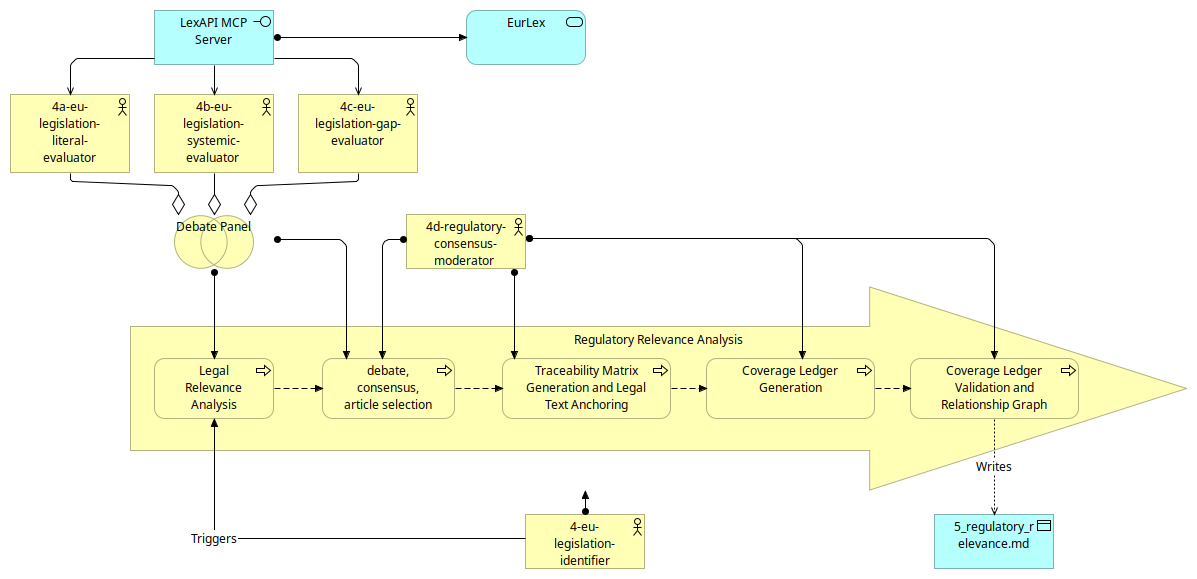
\includegraphics[width=1\textwidth]{Images/RegulatoryRelevanceAnalysis.png} 
  \caption{Overview of agent interaction in ``Regulatory Relevance Analysis'' step}
  \label{fig:reganalysisagentflow}
\end{figure}

Each evaluator independently retrieves the target regulation through \texttt{LexAPI} one article at a time and identifies potentially relevant articles. This is done to ensure that every article is analysed. Each one then explains their relevance through an operational anchor (the specific interview evidence, \texttt{OP-*} or \texttt{CON-*}), a legal bridge (how legal duty connects to that operational fact), and the operational ownership or reality (who performs the control) of the requirement. The evaluators also extract the complete set of requirements, restrictions, conditions, and obligations from each candidate article. Their proposals are then reviewed and challenged through a moderated debate. Only articles unanimously accepted by all three evaluators are retained as relevant. Split decisions are recorded as omitted candidate articles and are presented to the user for validation.

After having fixed the agreed articles, each approved atomic legal duty is recorded as a \texttt{REQ-*} requirement. The process then generates and validates the traceability matrix and links each identified \texttt{REQ-*} requirement to verified canonical legal-text identifiers (\textbf{R4}), and builds a Coverage Ledger, in which each entry receives a \texttt{COV-*} identifier. The corresponding approved operational-to-legal relationships are subsequently recorded as \texttt{REL-COV-*} entries (\textbf{R5}). A ledger entry provides the following information:

\begin{itemize}
    \item \textbf{Operational Fact Involved:} This is registered using the fact identifier mentioned in \ref{ContextDisc}.
    \item \textbf{Legal Requirement Affected:} Each legal requirement is given an identifier.
    \item \textbf{Evidence for Connection: } A statement from the interview that confirms an established connection.
    \item \textbf{Stakeholder Requirement Impact} : How this requirement affects the stakeholder.
    \item \textbf{Control Owner}: Ownership is classified as one of the following:
        \begin{itemize}
            \item \textbf{Directly Performed} - The stakeholder performs the relevant control;
            \item \textbf{Stakeholder-Constrained} - Another control or decision constrains the stakeholder;
            \item \textbf{Externally Owned} - Another team, supplier or organisation owns the control;
            \item \textbf{Not Evidenced / Unclear Owner } - Available evidence does not establish an owner.
        \end{itemize}
\end{itemize}
Afterwards, the ledger is validated so that it can be used to build relationship evidence. To be deemed valid:
\begin{itemize}
    \item Every operational fact documented from the interview  and concern must be connected to either:
    \begin{itemize}
        \item a legal requirement;
        \item a named operational-context stream.
    \end{itemize}
    \item Every included requirement must have a recorded operational chain, otherwise user clarification is requested.
    \item The coverage ledger entries become atomic relationship records. These specify the exact operational and legal endpoints, direction, meaning, evidence, and ownership state.
\end{itemize}

Following coverage resolution, the process maps the stakeholder to their employing organisation and then to the applicable law-defined entity or role group. These remain distinct concepts and are connected through evidence-backed \texttt{REL-ROLE-*} relationships. This prevents the model from incorrectly representing an individual stakeholder as the regulated entity merely because their organisation falls within the regulation's scope.

The resulting regulatory-relevance report is approved through six user gates covering relevant articles, omitted candidates, the legal index, legal-text identifiers, coverage relationships, and legal-role placement. Once approved, it becomes the evidence base for defining the stakeholder-specific viewpoint.

\subsection{Technology Selection and Overview View Generation}
\label{techSelect}

After \ref{regRevAnal}, the user is prompted to pick a technology. As can be seen in table \ref{tab:regulation-overview-archimate},
this phase contains three distinct agents, however, only one of them is used, depending on the technology choice made. This is because the view can be generated in three distinct ways:

\begin{enumerate}
    \item The first option is to generate the \texttt{.archimate} directly, using the agent to write the structured \ac{XML} syntax the modelling tool (Archi in this instance) can open. For this approach, agent \texttt{4e-a} is used alongside some specific skills (\texttt{archimate-xml-generator} and \texttt{archimate-symbol-validator}) for correct syntax, model understanding and validation.
    \item The second possibility is to generate a view using a different technology , LikeC4. This option was added as an academic experiment to the method. Agent \texttt{4e-b} achieves better results with LikeC4 when compared to direct \texttt{.archimate} generation. This is due to a key difference, which is that LikeC4 is an \ac{AAC} written in a custom \ac{DSL}. It was designed from the beginning to be integrated with \ac{LLM}s, and as a \ac{DSL}, it is significantly less verbose. However, the primary scope for this language is software architecture, not enterprise architecture.
    \item Lastly, there is also the possibility to pick pyArchimate. pyArchimate is a "Python library for programmatically reading, writing, and manipulating Open Group ArchiMate enterprise architecture models"\footnote{\label{fn:pyArchimate}pyArchimate library is available online in \url{https://pypi.org/project/pyArchimate/}}. It is included in the method as an attempt at using the best of both of the previously mentioned options. From the first choice, the preserved benefit is the Archimate output, which is the modelling language with \ac{EA} in scope. From the second approach, the \ac{AAC} advantage is kept intact. Therefore, instead of writing a high verbose file, the \ac{LLM} just needs to write a small python file that is easier to keep in context. The python script written by agent \texttt{4e-c} then outputs a \texttt{.archimate} file containing the model, justifying the inclusion of the skill \texttt{archimate-symbol-validator} for validation of the generated \ac{XML} syntax. 
\end{enumerate}

After having made a technology choice, the corresponding agent generates the overview view. This view is generated following these steps:
\begin{enumerate}
    \item \textbf{Verify the legal corpus:} Retrieve the consolidated binding text article by article;
    \item \textbf{Reject out-of-scope sources:} Recitals and generic legal headings cannot become model elements; 
    \item \textbf{Create legal requirement families:} Group binding duties into meaningful control domains;
    \item \textbf{Anchor legal duties:} Resolve every child requirement to verified Enacting Terms identifiers in the Traceability Matrix. Grouping elements receive the ordered, deduplicated list of their children's anchors;
    \item \textbf{Model containment and legal relationships:} Nest child requirements inside the corresponding requirement family. Only role-to-family or cross family relationships are drawn;
    \item \textbf{Add stakeholder context:} Add the approved stakeholder, employing organisation and law-defined entity or role chain to the view to improve readability and establish the legal perspective;
    \item \textbf{Validate graph integrity:} Every element needs an approved relationship, the stakeholder must be present and every element must be reachable from any other element;
    \item \textbf{Obtain user approval:} Confirm legal source completeness, obligation domain ,requirement families and the proposed overview map;
    \item \textbf{Materialize overview view:} The view is materialized to file, to be consumed by latter stages of the pipeline.
\end{enumerate}

The resulting artifact is therefore a technology-specific but semantically invariant baseline for all later stages. It represents the complete regulation-wide legal core through meaningful requirement families and their nested child obligations. The approved stakeholder to organisation to legal-role chain establishes the perspective of the stakeholder regarding that legal core without without treating the individual stakeholder and the regulated entity as one and the same.

Legal citations and verified traceability matrix \ac{ID}s are retained in model documentation (\textbf{R4}). Once fully approved, the overview becomes immutable. Later stages may create stakeholder-specific views, but they must preserve the legal core and stakeholder legal-role chain of the overview view.

\begin{table}[h]
\centering
\small
\begin{tabular}{p{5.2cm} p{5.5cm} p{3.5cm}}
\hline
\textbf{Agent} & \textbf{Used skill} & \textbf{Artifact produced} \\
\hline
4e-a-archimate-overview-modeler & archimate-xml-generator & 0\_regulation\_overview.archimate \\
 & archimate-symbol-validator &  \\
\hline
4e-b-likec4-overview-modeler & likec4-dsl & 0\_regulation\_overview.c4 \\
\hline
4e-c-pyarchimate-overview-modeler & pyarchimate-model-generator & 0\_regulation\_overview.py\\
 & archimate-symbol-validator & 0\_regulation\_overview.archimate  \\
\hline
 4e-a, 4e-b and 4e-c& regulation-overview-designer &  \\
 & legal-text-anchor-resolver &  \\
 & stakeholder-legal-role-mapper &  \\
 & regulatory-view-structure &  \\
 & connected-view-validator &  \\
\hline
\end{tabular}
\caption{Contextualized regulation overview using ArchiMate XML.}
\label{tab:regulation-overview-archimate}
\end{table}

\subsection{Viewpoint Scope}
\label{vpScope}

Following the ``Regulatory Relevance Analysis'', the ``Viewpoint Scope'' is responsible for answering the question : ``Which parts of the stakeholder’s operational reality and the regulation should be represented, and why?''. No new legal requirements or operational facts are created during this step. The agent responsible uses the skills observable in table \ref{tab:viewpoint-scope} to filter and organise the approved evidence from earlier steps. It determines the boundary of the viewpoint trough chaining requirements to the stakeholder. A legal requirement is included only when it has a recorded operational chain to the stakeholder. Requirements that are applicable to the organisation, without a documented impact on the stakeholder's work, remain outside the scope (\textbf{R6 and R5}).

\begin{table}[!bt]
\centering
\small
\begin{tabular}{p{5.2cm} p{5.5cm} p{3.5cm}}
\hline
\textbf{Agent} & \textbf{Used skill} & \textbf{Artifact produced} \\
\hline
5-stakeholder-viewpoint-scoper &
viewpoint-scope-definer &
6\_viewpoint\_scope.md \\
 &
stakeholder-footprint-coverage &
 \\
 &
evidence-grounded-relationship-ledger &
 \\
 &
regulatory-view-structure &
 \\
 &
connected-view-validator &
 \\
\hline
\end{tabular}
\caption{Viewpoint scope and justification step.}
\label{tab:viewpoint-scope}
\end{table}

The agent groups included material from previous steps (operational footprint, relevant articles, stakeholder classification, coverage and relationship ledger, and regulation overview baseline) into coherent operational streams (\textbf{R1}). Examples of this, when applied to the \ac{DORA} regulation from the viewpoint of a developer, are ``Protection and Change'', ``Resilience Testing'', ``Detection and Continuity'', among others streams. Each group is further distinguished as Governance, Administrative, or Technical. Non-regulatory work is retained in a role-specific operational-context stream rather than being incorrectly presented as a legal duty.

Ownership remains an important distinction in this step. A directly performed requirement may later be represented as a stakeholder realisation. A stakeholder-constrained, externally owned or of unclear ownership requirement must be shown through an appropriate dependency, role, approval or constraint.

These groups are also proposed as the future views to be generated. Every candidate view must contain the stakeholder, include only approved relationships, have no isolated elements, and every element must be reachable from any other element. If a proposed view has disconnected parts, it is split into meaningful separate views (\textbf{R1}). During the process, the user must approve:
\begin{itemize}
    \item The defined scope boundary;
    \item Included requirements;
    \item Operational streams;
    \item The connectivity of each proposed view;
    \item Any eventually required split.
\end{itemize}

\subsection{Viewpoint Generation}

The ``Viewpoint Generation'' step converts the scope approved in the previous phase into the formal ArchiMate viewpoint and an authoritative view graph. The viewpoint defines exactly what later artefacts are allowed to represent (strengthens \textbf{R3}).

The agent takes the approved scope, Coverage Ledger, relationship evidence, and immutable Regulation Overview baseline. Then, for each view, it defines:
\begin{itemize}
    \item Purpose and stakeholder perspective.
    \item Included concerns and operational streams.
    \item Allowed ArchiMate elements and relationships.
    \item Requirement-family structure and nesting.
    \item Visual rules and layout constraints.
    \item Evidence (\textbf{R5}), ownership safeguards (\textbf{R6}), and legal-text documentation (\textbf{R4}). 
\end{itemize}

The overview view remains the same generated in \ref{regRevAnal}. It preserves the regulation-wide legal core. Other views will represent the narrower the narrower, stakeholder specific operational scope.

An important output of this step is \texttt{7\_view\_graph.json}, one of the outputs present in table \ref{tab:viewpoint-generation}. It is an authoritative machine-readable graph contract for all later outputs (narrative, slides and model generation). It records:
\begin{itemize}
    \item Every allowed node and its view membership.
    \item Every approved \texttt{REL-*} relationship (these include endpoints, direction, meaning, evidence, and visibility).
    \item Requirement family containment and visual nesting.
    \item The stakeholder anchor in every view.
    \item Ownership rules, such as preventing an externally owned requirement from being represented as stakeholder realisation.
\end{itemize}

The generated viewpoint also perpetuates every restriction defined in the \ref{vpScope} down to the view level. Before materializing the viewpoint to file, the user must validate the metamodel scope defined by the viewpoint (allowed ArchiMate concepts, relationships and visual rules) as well as the view graph (each view's nodes, relationships, nesting and connectivity result).
The resulting viewpoint specification and graph become the fixed contract used to generate the explanatory text, slide diagrams, and final model (\textbf{R3}).

\begin{table}[h]
\centering
\small
\begin{tabular}{p{5.2cm} p{5.5cm} p{3.5cm}}
\hline
\textbf{Agent} & \textbf{Used skill} & \textbf{Artifact produced} \\
\hline
6-viewpoint-materializer &
viewpoint-creator &
7\_viewpoint.md \\
 &
viewpoint-materializer &
7\_view\_graph.json \\
 &
stakeholder-footprint-coverage &
\\
 &
evidence-grounded-relationship-ledger &
\\
 &
regulatory-view-structure &
\\
 &
connected-view-validator &
\\
\hline
\end{tabular}
\caption{Viewpoint generation step.}
\label{tab:viewpoint-generation}
\end{table}

\subsection{Textual View Explanation}

The viewpoint and graph can be used to convey information in a multitude of ways. One of them, materialized in this stage, is the \texttt{view\_explanation}. The agent of this phase, represented in \ref{tab:textual-view-explanation}. It serves two purposes at once: To explain how the regulation affects the daily work of the stakeholder and to explain how to read the corresponding architectural views (\textbf{R1}). For this, the agent uses the viewpoint and the view graph created in the previous step as a source of truth, not adding, removing or changing any nodes or relationships.

\begin{table}[h]
\centering
\small
\begin{tabular}{p{5.2cm} p{5.5cm} p{3.5cm}}
\hline
\textbf{Agent} & \textbf{Used skill} & \textbf{Artifact produced} \\
\hline
7-view-narrative-explainer &
view-narrative-explainer &
1\_view\_explanation.md \\
 &
stakeholder-footprint-coverage &
\\
 &
evidence-grounded-relationship-ledger &
\\
 &
regulatory-view-structure &
\\
 &
connected-view-validator &
\\
\hline
\end{tabular}
\caption{Textual view explanation step.}
\label{tab:textual-view-explanation}
\end{table}
The explanation is generated in a per-view basis, starting with the regulation wide overview view. This explanation each stakeholder-specific stream, such as governance, operational administration, or technical work. Then, for each other view, the explanation describes:
\begin{itemize}
    \item The view's purpose and stakeholder concern;
    \item Relevant operational tasks, systems and dependencies;
    \item Applicable requirement families and granular legal requirements;
    \item Ownership state of each legal effect;
    \item Relations between elements.
\end{itemize}
These topics cover the narrative walk-through of the operational and regulatory context. In addition, every stakeholder-specific view contains an explicit ``How to read this view'' subsection. It explains:
\begin{itemize}
    \item every visible box, including its ArchiMate type, what it represents, why it is present, and whether it is nested within a requirement family;
    \item every visible arrow, including its source and target, relationship type, evidence-backed meaning, and why it is represented visibly;
    \item semantic-only composition or aggregation relationships, which are communicated through nesting rather than an internal arrow;
    \item the route from the stakeholder to the relevant operational elements, dependencies, external roles, and requirement families;
    \item external actors, systems, approval gates, and unclear-owner requirements, explaining why they remain outside the stakeholder's direct control;
    \item the distinction between work directly performed by the stakeholder and work that is constrained, externally owned, or not evidenced.
\end{itemize}
Before being materialized to file the user must approve, for each view, the view name and the view description.
The final artifact also contains a layer-by-layer explanation of the ArchiMate concepts used across the viewpoint and a complete traceability table. This table connects each Coverage Ledger entry to its operational source, requirement family, legal requirement, ownership state, representing element or external role, and operational meaning.


\subsection{Markdown Slide Diagrams}

The next stage is ``Markdown Slide Diagram'' generation. The artifact observable in \ref{tab:markdown-slide-diagrams} is produced by the agent of this step, who turns the approved viewpoint, graph and textual explanation into a presentation-style visual document. The main goal of this step is to present an accessible, condensed visual summary of each approved view (\textbf{R1}). The complete view is conveyed by the diagram together with its supporting tables; the diagram itself is not an exact graphical projection of every element and relationship.

\begin{table}[b]
\centering
\small
\begin{tabular}{p{5.2cm} p{5.5cm} p{3.5cm}}
\hline
\textbf{Agent} & \textbf{Used skill} & \textbf{Artifact produced} \\
\hline
8-informal-diagram-designer &
informal-markdown-diagram-designer &
2\_slide\_diagrams.md \\
 &
stakeholder-footprint-coverage &
 \\
 &
evidence-grounded-relationship-ledger &
 \\
 &
regulatory-view-structure &
 \\
 &
connected-view-validator &
 \\
\hline
\end{tabular}
\caption{Markdown slide diagrams step.}
\label{tab:markdown-slide-diagrams}
\end{table}

The output begins with the slide for the overview view. Its \texttt{ASCII} diagram is a compressed representation of the immutable legal core. It is followed by one slide for each stakeholder-specific view defined in the viewpoint graph.

Each stakeholder-specific slide contains a condensed \texttt{ASCII} diagram sketch. It shows the stakeholder, the principal operational path, relevant systems or external dependencies, and every requirement family as a labelled group. Accompanying the sketch are two supporting tables:
\begin{itemize}
    \item \textbf{Component Breakdown:} Listing every granular requirement within each requirement family, together with readable legal citations, ownership state, and operational relevance;
    \item \textbf{Relationship Inventory:} Recording every approved relationship by its readable source, meaning, target, ArchiMate type, and ownership.
\end{itemize}
Lastly, each slide contains an Operational Takeaway in plain language, summarising the direct work, constraints, dependencies, and potential operational or visibility limitations of the stakeholder.

Before being commited to file, the user must approve each \texttt{ASCII} slide individually, including the detailed information retained in the accompanying tables.

\subsection{View Generation}

The view generation is the phase where viewpoints are materialized in the form of views. The architecture model that a modelling tool can open, inspect, reuse and refine. It is not intended to be a finished product, but to be used as a starting point to be improved over iterative efforts. The step consists of only a single agent, despite three distinct agents being present, as shown in table \ref{tab:viewpoint-generation}. This is because the views can be generated in three distinct ways, the same way as in \ref{techSelect}.

Despite the choice made on step \ref{techSelect}, the user is prompted to choose one of these three options. Regardless of the technology option, the agent associated with the choice always requires the same input:
The overview view, viewpoint, view graph, textual view explanation and the condensed slides.
From these inputs, the graph is the absolute authority while the narrative and the condensed slides help explain and organise the model.
The process then works as follows:

\begin{enumerate}
    \item The agent creates the model elements from the approved graph;
    \item Requirement hierarchy is preserved. Each requirement group is a meaningful parent ArchiMate Requirement or Constraint, with its child requirements are visually nested within it (\textbf{R1});
    \item Approved relationships are materialized with their exact source, target, direction, and ArchiMate type. A stakeholder may realise a requirement only where ownership is Directly performed (\textbf{R5});
    \item The overview view is copied and the stakeholder-specific native views are created. Every view includes the stakeholder and contains no isolated elements. Arrows are only omitted where visual nesting communicates containment;
    \item Citations, ownership metadata, and traceability matrix \ac{ID}s are stored in element descriptions (\textbf{R4});
    \item Output is validated in the selected technology:
    \begin{itemize}
        \item Archimate \ac{XML} checks structure, folders, diagram objects, connections and coordinates.
        \item LikeC4 checks \ac{DSL} syntax, scoped references and rendered views.
        \item pyArchimate validates relationship legality, executes the generator script.
    \end{itemize}
    \item The proposed thematic view layouts are presented to the user for approval before persistence;
    \item The generated model is checked against the graph. Missing nodes, extra relationships, broken containments, disconnected views or an altered overview view cause model rejection (\textbf{R3}).
\end{enumerate}

\begin{table}[h]
\centering
\small
\begin{tabular}{p{5.2cm} p{5.5cm} p{3.5cm}}
\hline
\textbf{Agent} & \textbf{Used skill} & \textbf{Artifact produced} \\
\hline
9a-archimate-model-generator & archimate-xml-generator & 3\_view\_model.archimate \\
 & archimate-symbol-validator &  \\
\hline
9b-likec4-model-generator & likec4-dsl & 3\_view\_model.c4 \\
\hline
9c-pyarchimate-model-generator & pyarchimate-syntax-reference & 3\_view\_model\_pyarchimate.py\\
 & archimate-symbol-validator & 3\_view\_model\_pyarchimate.archimate \\
\hline
9a, 9b and 9c & stakeholder-footprint-coverage &  \\
 & evidence-grounded-relationship-ledger &  \\
 & regulatory-view-structure &  \\
 & connected-view-validator &  \\
\hline
\end{tabular}
\caption{View generation using ArchiMate XML.}
\label{tab:view-generation-archimate}
\end{table}


\subsection{Cross-Artifact Reconciliation}

The last step in the pipeline is ``Cross-Artifact Reconciliation''.  All necessary knowledge basis are present in table \ref{tab:cross-artifact-reconciliation}. This stage is responsible for ensuring that all generated artefacts depict the same information (\textbf{R3}). The agent responsible for this phase compares:
\begin{itemize}
    \item Overview view;
    \item Viewpoint and the graph;
    \item Textual explanation;
    \item Explicative Slides; 
    \item The model;
    \item Traceability Matrix.
\end{itemize}

\begin{table}[bt]
\centering
\small
\begin{tabular}{p{5.2cm} p{5.5cm} p{3.5cm}}
\hline
\textbf{Agent} & \textbf{Used skill} & \textbf{Artifact produced} \\
\hline
10-view-cross-artifact-reconciler &
view-cross-artifact-reconciler &
Audit report \\
 &
legal-text-anchor-resolver &
View Updates \\
 &
stakeholder-footprint-coverage &
\\
 &
evidence-grounded-relationship-ledger &
\\
 &
regulatory-view-structure &
\\
 &
connected-view-validator &
\\
\hline
\end{tabular}
\caption{Cross-artifact reconciliation step.}
\label{tab:cross-artifact-reconciliation}
\end{table}

This is important because each artefact can appear valid on its own while contradicting another. For example, a narrative may describe a developer as constrained by a control while the model incorrectly depicts them as directly realising it, or a requirement could be renamed in slides but retain its original legal anchor in the model.
Then validation happens in the following step by step manner:
\begin{enumerate}
    \item Reads the approved graph as the ground truth;
    \item Verifies the overview view against the traceability matrix to check the legal anchors;
    \item Checks that each in-scope requirement has an operational chain;
    \item Compares the narrative, slides, and model against the approved view elements and relationships;
    \item Validates the technology-specific syntax of the model, references, containment, and diagram connections;
    \item Produces a discrepancy report if anything differs;
    \item Presents the user with a confirmation gate, so that nothing is modified without permission;
    \item Applies only the user approved corrections;
    \item Reruns the audit.
\end{enumerate}

The gain is assurance: the final model, explanation, and slides can be used by different readers without silently communicating incompatible claims. These artifacts also support each other. If the stakeholder is not proficient in reading Archimate diagrams, condensed slides and explicative text may help with correctly interpreting the views.